% Rebuild:
%   pdflatex -output-directory=docs docs/pipeline.tex
%   pdftocairo -svg docs/pipeline.pdf docs/pipeline.svg
\documentclass[border=6pt]{standalone}
\usepackage{tikz}
\usetikzlibrary{arrows.meta,calc,positioning,backgrounds}
\usepackage{xcolor}
\tikzset{
  background rectangle/.style={fill=white, rounded corners=10pt},
  inner frame sep=9pt,
}
\begin{document}
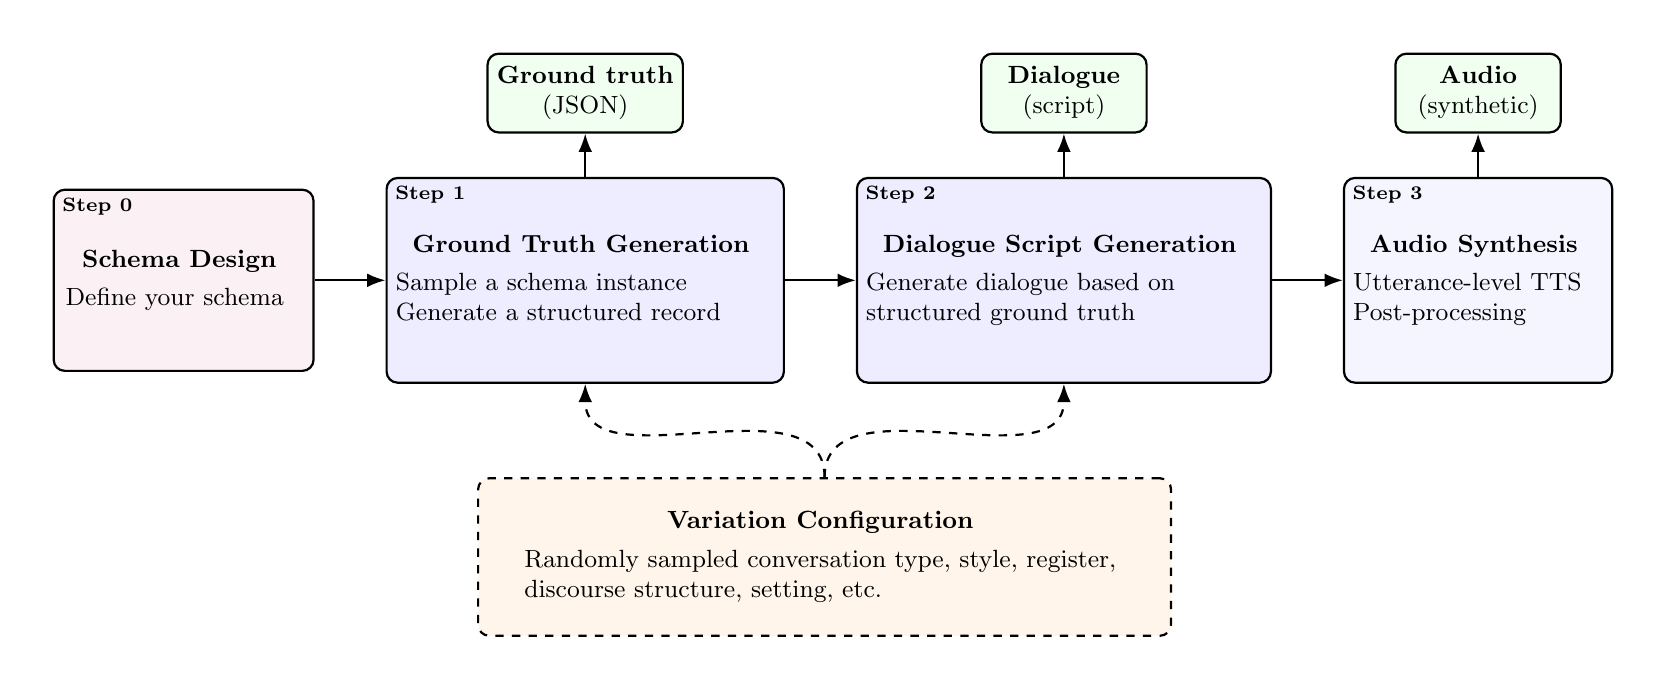
\begin{tikzpicture}[show background rectangle,
			node distance=1.2cm and 0.9cm,
			>=Latex,
			font=\small,
			prepbox/.style={
				draw,
				rounded corners,
				thick,
				align=center,
				minimum width=3.3cm,
				minimum height=2.3cm,
				fill=purple!6
			},
			stepbox/.style={
				draw,
				rounded corners,
				thick,
				align=center,
				minimum width=3.5cm,
				minimum height=2.6cm,
				fill=blue!7
			},
			audiobox/.style={
				draw,
				rounded corners,
				thick,
				align=center,
				minimum width=3.3cm,
				minimum height=2.6cm,
				fill=blue!4
			},
			cfgbox/.style={
				draw,
				rounded corners,
				thick,
				dashed,
				align=left,
				minimum width=8.8cm,
				minimum height=2.0cm,
				fill=orange!8
			},
			outputbox/.style={
				draw,
				rounded corners,
				thick,
				align=center,
				minimum width=2.1cm,
				minimum height=1.0cm,
				fill=green!6
			},
			mainarrow/.style={thick, ->},
			influarrow/.style={thick, dashed, ->}
			]
			
			% Step 0
			\node[prepbox] (schema) {
				\begin{tabular}{@{}l@{}}
					\multicolumn{1}{c}{\textbf{Schema Design}}\\[1mm]
					\small Define your schema
				\end{tabular}
			};
			
			% Step 1
			\node[stepbox, right=of schema] (step1) {
				\begin{tabular}{@{}l@{}}
					\multicolumn{1}{c}{\textbf{Ground Truth Generation}}\\[1mm]
					\small Sample a schema instance\\
					\small Generate a structured record
				\end{tabular}
			};
			
			% Step 2
			\node[stepbox, right=of step1] (step2) {
				\begin{tabular}{@{}l@{}}
					\multicolumn{1}{c}{\textbf{Dialogue Script Generation}}\\[1mm]
					\small Generate dialogue based on\\
					\small structured ground truth
				\end{tabular}
			};
			
			% Step 3
			\node[audiobox, right=of step2] (step3) {
				\begin{tabular}{@{}l@{}}
					\multicolumn{1}{c}{\textbf{Audio Synthesis}}\\[1mm]
					\small Utterance-level TTS\\
					\small Post-processing
				\end{tabular}
			};
			
			% Step labels (corner tags)
			\node[anchor=north west, font=\scriptsize\bfseries] at (schema.north west) {Step 0};
			\node[anchor=north west, font=\scriptsize\bfseries] at (step1.north west) {Step 1};
			\node[anchor=north west, font=\scriptsize\bfseries] at (step2.north west) {Step 2};
			\node[anchor=north west, font=\scriptsize\bfseries] at (step3.north west) {Step 3};
			
			% Outputs
			\node[outputbox, above=0.55cm of step1] (o1) {\textbf{Ground truth}\\(JSON)};
			\node[outputbox, above=0.55cm of step2] (o2) {\textbf{Dialogue}\\(script)};
			\node[outputbox, above=0.55cm of step3] (o3) {\textbf{Audio}\\(synthetic)};
			
			% Config
			\coordinate (mid12) at ($(step1)!0.5!(step2)$);
			\node[cfgbox, below=2.5cm of mid12] (cfg) {
				\begin{tabular}{@{}l@{}}
					\multicolumn{1}{c}{\textbf{Variation Configuration}}\\[1mm]
					\small Randomly sampled conversation type, style, register,\\
					\small discourse structure, setting, etc.\\
				\end{tabular}			
			};
			
			% Pipeline arrows
			\draw[mainarrow] (schema) -- (step1);
			\draw[mainarrow] (step1) -- (step2);
			\draw[mainarrow] (step2) -- (step3);
			
			% Output arrows
			\draw[mainarrow] (step1) -- (o1);
			\draw[mainarrow] (step2) -- (o2);
			\draw[mainarrow] (step3) -- (o3);
			
			% Influence arrows
			\draw[influarrow] (cfg.north) to[out=90,in=-90] (step1.south);
			\draw[influarrow] (cfg.north) to[out=90,in=-90] (step2.south);
			
		\end{tikzpicture}
\end{document}
